\documentclass[10pt, conference, compsocconf]{IEEEtran}

\usepackage{capt-of}
\usepackage{graphicx}
\usepackage{subfig}
\usepackage{booktabs}
\usepackage{multirow}
\usepackage{siunitx}
\usepackage{multicol}
\usepackage{array}
\usepackage{amsmath}
\newcommand{\nltable}[2][c]{%
  \begin{tabular}[#1]{@{}c@{}}#2\end{tabular}}
\newcommand{\wave}{\raise.17ex\hbox{$\scriptstyle\mathtt{\sim}$}}

\newcolumntype{C}[1]{>{\centering\let\newline\\\arraybackslash}m{#1}}

\begin{document}
\bstctlcite{IEEEexample:BSTcontrol}

\title{Approach of Matrix Multiplication on Cloud Distributed System}


\author{\IEEEauthorblockN{Myungjun Son}
\IEEEauthorblockA{Department of Computer Science\\
Kookmin University\\
Seoul, South Korea\\
smj8612@kookmin.ac.kr}
\and
\IEEEauthorblockN{Kyungyong Lee}
\IEEEauthorblockA{Department of Computer Science\\
Kookmin University\\
Seoul, South Korea\\
leeky@kookmin.ac.kr}
}

% make the title area
\maketitle

\begin{abstract}
Abstract
\end{abstract}

\IEEEpeerreviewmaketitle

\section{Introduction}\label{sec:intro}
Big data analytics systems are deployed in cloud computing environments to process ever-increasing dataset while guaranteeing stable operations; scalability and fault-tolerance from the perspective of infrastructure. To satisfy application demands from distinct use cases, cloud computing service providers offer various types of instances that applications can run. Using those resources, most big data platforms are deployed in a scale-out manner. As managing distributed datasets and tasks running on large-scale machines are challenging, abstractions of distributed datasets and resources are crucial to let application developers focus on tasks that really matter. Many systems are proposed to provide a simple and easy interface to handle large-scale datasets, to name a few, Hadoop~\cite{hadoop}, Spark~\cite{spark}, and recently TensorFlow~\cite{tensorflow}.

To extract valuable insights from massive dataset, matrix multiplication is widely used. In recommendation systems, for example, the core computation kernel of matrix factorization algorithms, such as SVD and NMF~\cite{nmf}, is matrix-matrix multiplication. The matrix-vector multiplication is the core kernel in page-rank algorithm when using the power method to get principle eigen vectors~\cite{pagerank}. In order to build a cost efficient cloud environment that runs data mining tasks with distributed matrix computation kernel, it is crucial to estimate the kernel task overhead on different cloud computing instances with distinct matrix size. 

To understand the characteristics of matrix multiplication performance on a distributed cloud computing environment, we analyzed the performance of dense matrix multiplication with diverse input sizes and formations on distinct cloud computing instances. In the experiments, we multiply two square matricies with the number of rows being 10000, 20000, and 30000 on AWS EC2 \textit{R4, T2, M4, C4, G2} instances with size of \textit{2xlarge}. We use Apach Spark MLLib BlockMatrix library~\cite{spark-mm} to conduct the experiments with four machines that have OpenBlas installed. 

Figure~\ref{fig:different-instance-types} shows the normalized latency to the fastest completing instance type in the gray bar. As shown in the figure, as the input matrix size differs, the best performing instance type also differs - no globally optimal instance type. If we consider the price factor of each instance, the performance difference even gets bigger as shown in the red star mark. Furthermore, as shown in the Figure~\ref{fig:instance-blocks-sizes-compare}, multiplying two non-sqaure matricies shows siginificantly different performance comparing to the square matrix multiplication though the number of compute operation is the same - i.e., the number of (left matrix rows $\times$ left matrix columns $\times$ right matrix columns).

\begin{figure}[!ht]
  \centering
  \subfloat[Performance of different instance types of 2xlarge]{\label{fig:different-instance-types}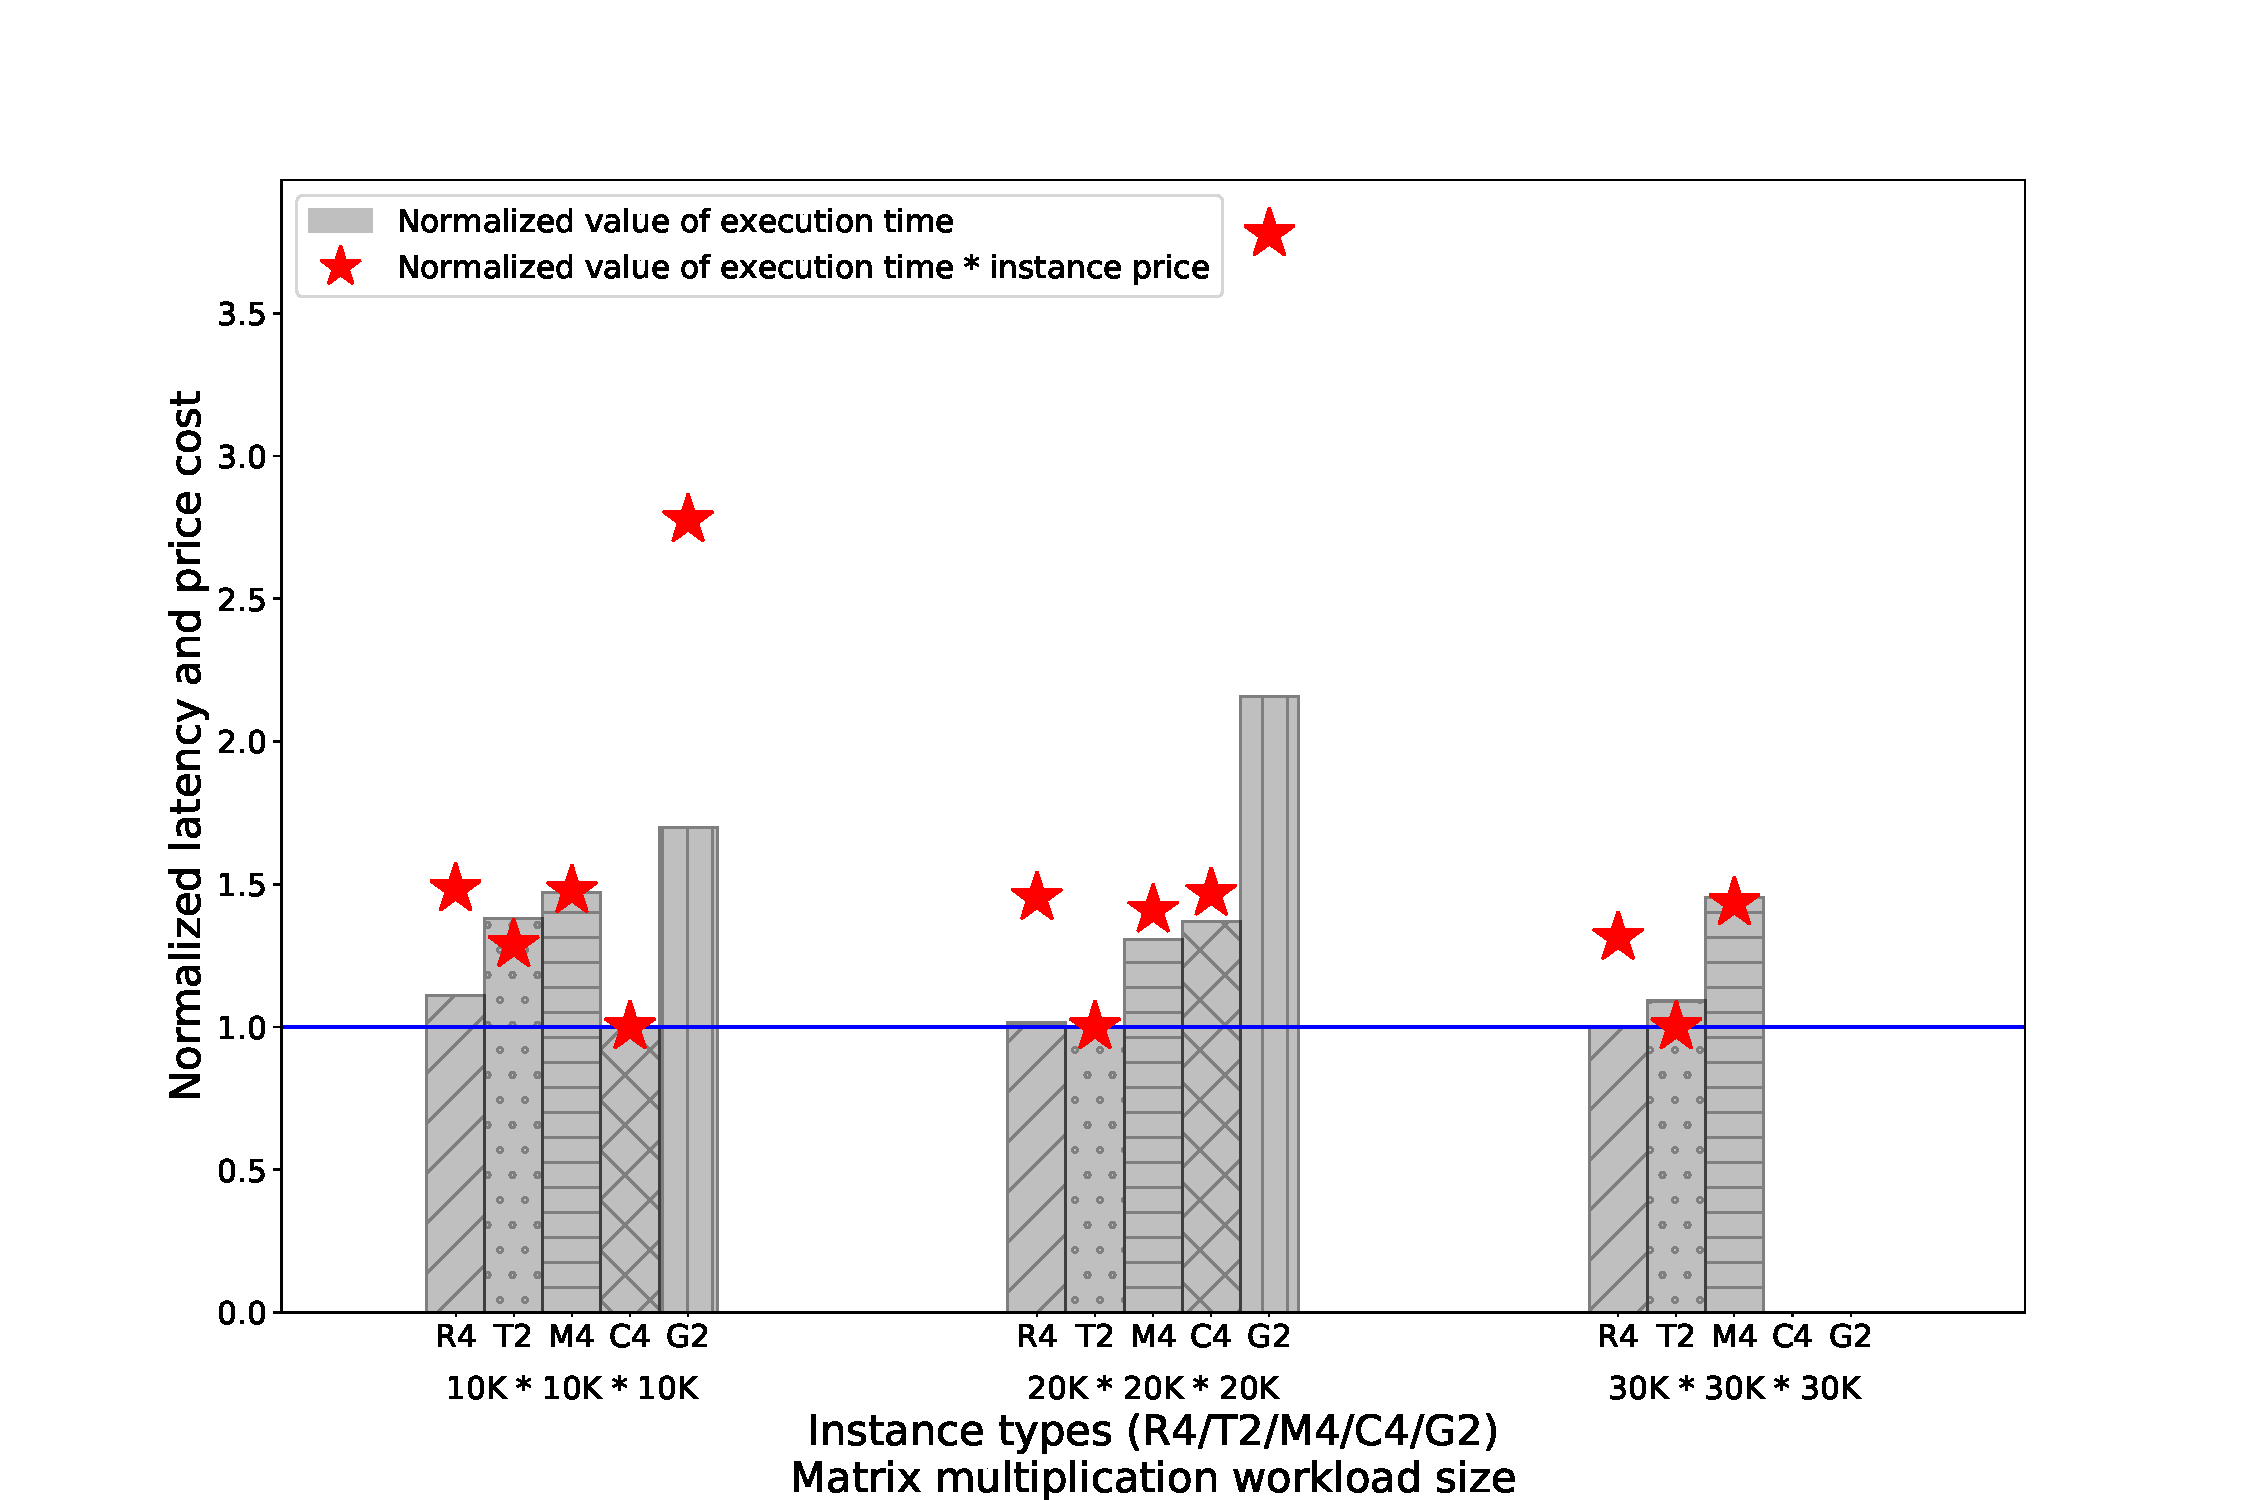
\includegraphics[width=0.5\textwidth]{figures/instance-2xl-compare.pdf}}\\
  \subfloat[Performance of different matrix shapes]{\label{fig:different-matrix-shapes}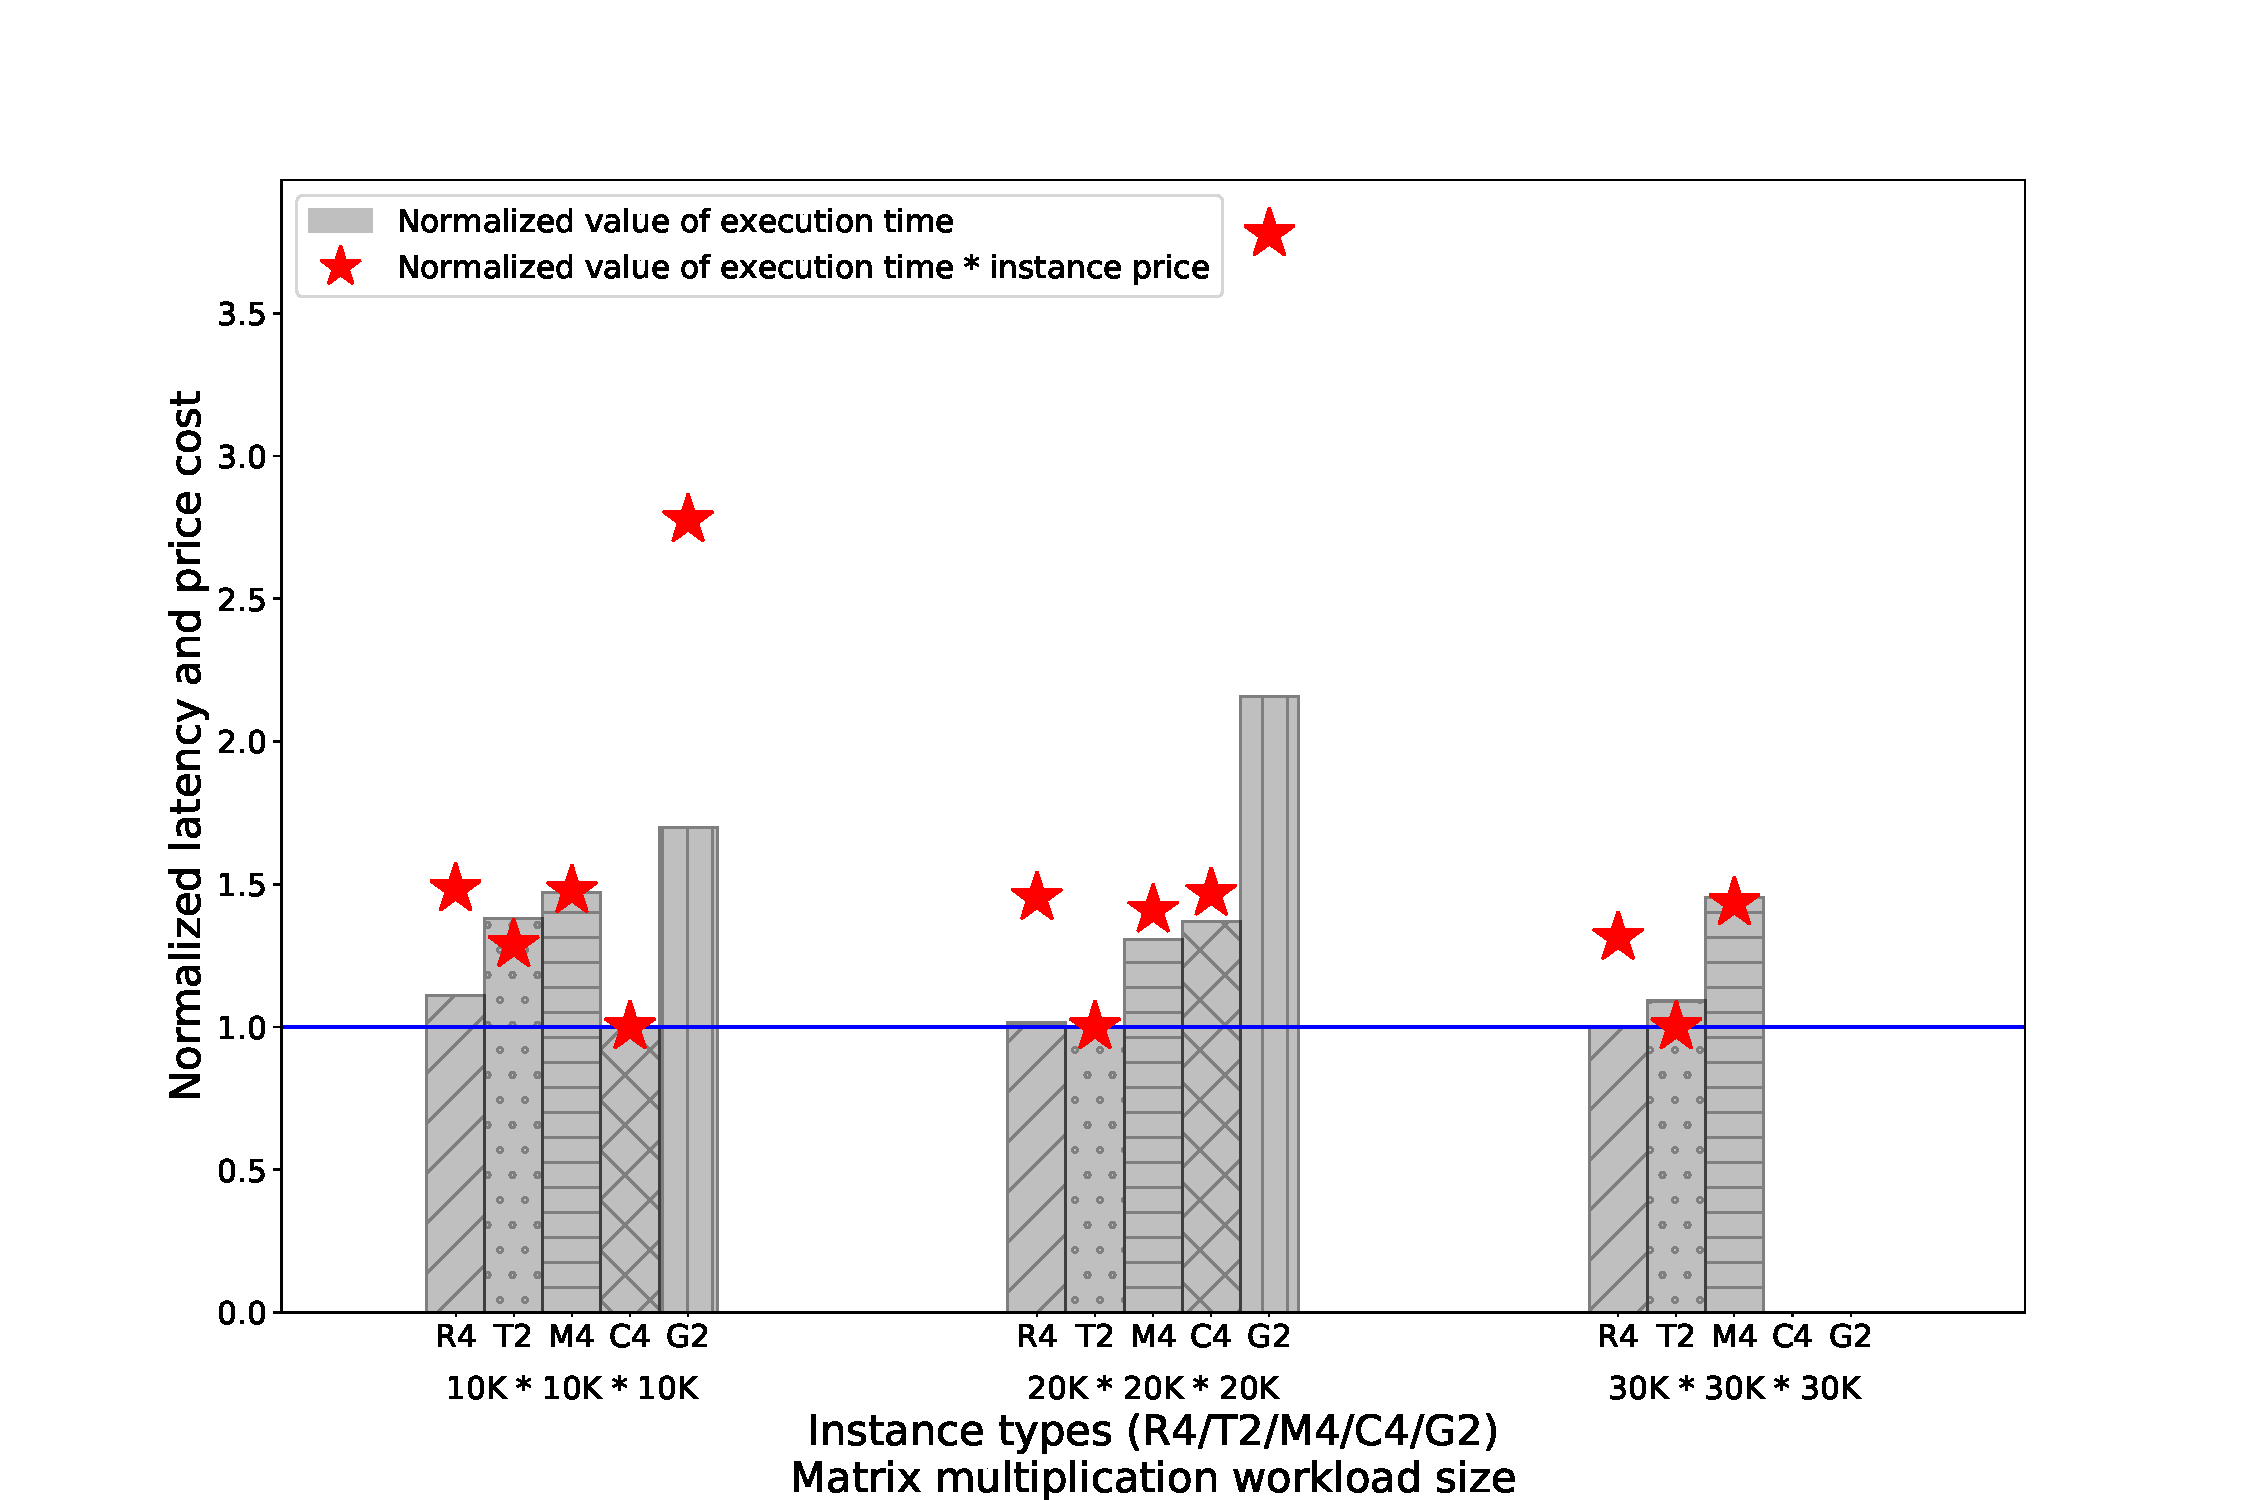
\includegraphics[width=0.5\textwidth]{figures/instance-2xl-compare.pdf}}
  \caption{\label{fig:instance-blocks-sizes-compare}. The normalized value of latency with respect to different instance types and input matrix shapes - the lower, the better.}
\end{figure}

Despite of the importance of the matrix multiplication when running machine learning tasks, performance analysis and modeling in a distributed cloud computing environment are not thoroughly conducted yet. Few works focused on predicting data mining algorithm performance on a cloud comptuing environment - Ernest~\cite{ernest}, CherryPick~\cite{cherrypick}, and PARIS~\cite{paris}. The proposed methods rely on a scale-based sampling method to estimate the latency to complete original large input size, and they show poor accuracy when predicting distributed matrix multiplication task running time as they fail to catpture the nature of distrbuted matrix computation. Performance modeling and prediction on a single machine with multiple cores are well studied in literature with hardware optimized libraries, such as OpenBLAS, but previous works generally do not consider network and IO overhead that can be additional significant overhead in a distributed cloud computing environment.

In this paper, we propose MPC (\textbf{M}atrix Multiplication \textbf{P}erformance Predictor for \textbf{C}loud Computing) to provide accurate latency prediction while performing multiplication of arbitrary shape and size of matricies on diverse cloud computing resources. MPC profiles the latency to perform multiplication on two unit-block matricies on diverse cloud computing resources. In order to represent the profiled unit-block latency results, MPC builds a model with XXXX followed by bayesian optimization to find the optimal hyper parameters to minimize the modeling error. In the step of prediction of arbitrary size matrix multiplication, MPC proposes to disassemble the input matricies into blocks that worker nodes can operate, and the latency to multiply each block matrix is made by using the model built from the unit-block matricies. MPC eventually stitches the blocks to conjecture the overall task completion time.

% summarize the result
% itemize the contributions

\section{Matrix Multiplication on a Distributed Computing Environment}\label{sec:distributed-matrix-computation}
% explain how the matrix computation happens in spark - mention the step of shuffle, compute, reduce
% How block matrix multiplication happens with the overhead (shuffle, compute, reduce)
Optimization of distributed matrix multiplication is well studied in literature. In the HPC community, many works focused on minimzing communication cost using MPI model. Representative works include SUMMA~\cite{summa} and CARMA~\cite{carma}. Despite of the performance optimality of the methods, they have limitations regarding the programmability, scalability, and robustness comparing to general purpose big-data analytics systems, such as Spark~\cite{spark} and Hadoop~\cite{hadoop}, especially on a shared cloud computing environment.

0Apache Spark is an open source big-data analytics platform. The primary abstraction in Spark is Resilient Distributed Dataset(RDD), which represents a read-only collection of objects partitioned across a set of machines. Spark manages large-scale data using partitions that helps parallelize distributed data processing while guaranteeing the fault-tolerance with lineage and task execution optimization with lazy evaluation~\cite{spark}.

In Spark, matrix-related linear algebric operations are supported in the MLLib library~\cite{spark-mm} with various matrix partitioning heuristics (row-, column-, and block-based) and a set of distributed operation APIs on the matrix. To multiply two matricies, Spark MLLib automatically identifies the optimal way of task distribution based on the input matrix partitioning scheme and uses Scala Breeze library to execute multiplication. Let us give an example of multiplying two matricies, $C = A \times B$. If $A$ is row-partitioned and $B$ is column-partitioned, the cartesian product is performed for each row block of $A$ and column block of $B$. If both $A$ and $B$ are block-partitioned, the block dimension of result matrix, $C$, is decided by considering the number of workers and input block dimensions. A work node that is responsible for each resulting block fetches all the necessary blocks from $A$ and $B$ to execute multiply operation locally.

\begin{figure}
  \centering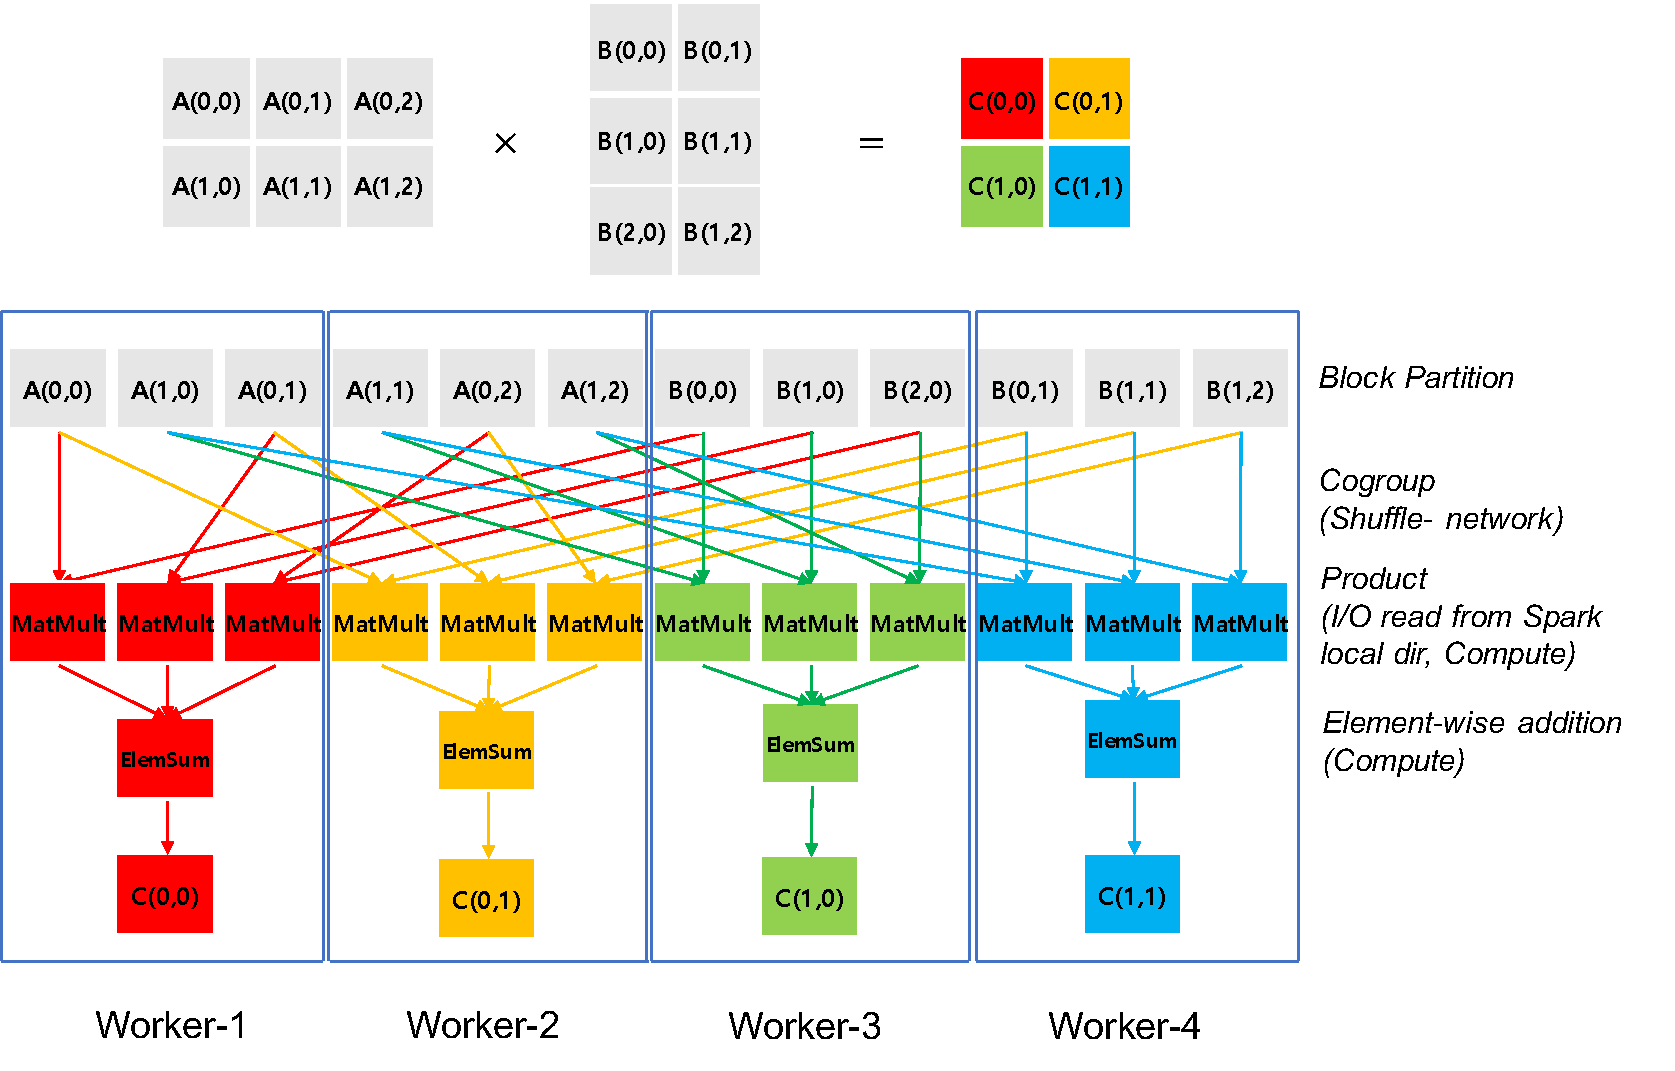
\includegraphics[width=0.45\textwidth]{figures/matmult-overhead-non-square.pdf}\caption{Block-based distributed matrix multiplication and its overhead in each step. Network, IO, and CPU are principal resources for the execution.}\label{fig:matmul-with-overhead}
\end{figure}
Figure~\ref{fig:matmul-with-overhead} shows an example of block-based matrix multiplication. A left matrix, $A$, is block-partitioned by $2 \times 3$, a right matrix, $B$, is partitioned by $3 \times 2$, and the result matrix, $C$, is partitioned by $2 \times 2$. In Spark, a \textit{cogroup} operation by the result matrix block index allows a worker node that is responsible for a result block to collect necessary left and right matrix blocks. During \textit{cogroup} operation, network overhead is dominant. After collecting all necessary blocks, each worker node performs a product operation followed by an element-wise addition. In the step, I/O overhead to read the fetched blocks from a \textit{local.dir} location and compute overhead dominates.

\subsection{Distributed Matrix Multiplication Overhead Modeling}\label{sec:overhead-modeling}
Dense matrix multiplication is widely known as a CPU intensive task, but other resource overheads become non-negligible when it is executed on a large-scale distributed computing environment, such as Spark. To qualitatively understand the characteristics of a distributed matrix multiplication task, we summarize overheads when a task is executed on Apach Spark. Let us assume the number of rows of a left matrix as $N$, the number of columns of a left matrix (or the number of rows of a right matrix) as $K$, and the number of columns of a right matrix as $M$. Accordingly, the result matrix size is $N \times M$. Left, right, and result matricies are block-partitioned whose partition size is expressed in the lowercase letter ($n$, $k$, and $m$, where $N \geq n$, $M \geq m$, and $K \geq k$). 

\textbf{Shuffle}: A worker node that is responsible for computing an output matrix block of size $n \times m$ has to fetch blocks from left and right matricies with the size of $n \times K$ and $K \times m$, respectively. If a worker node does not contain required blocks locally, it has to fetch them from remote machines that incurs network overhead. Assuming uniform block distribution among workers, the network overhead in the shuffle phase can be expressed as Equation~\ref{eq:shuffle-overhead}.
\begin{equation}\label{eq:shuffle-overhead}
  BlockFetchOverhead_{n \times m} \propto \sum\limits_{i=1}^{\frac{K}{k}} n \times k + k \times m
\end{equation}

\textbf{Compute}: After a shuffle step completes, a worker node performs multiplication of fetched blocks followed by element-wise addition. In order to perform multiplication, the blocks have to be read from a Spark local directory (\textit{spark.local.dir} configuration) that is generally set as an disk. Thus, the IO read overhead is same as the shuffle overhead and expressed as Equation~\ref{eq:shuffle-overhead}.

After loading the input matrix blocks, each worker node executes a multiplication task whose overhead is expressed as Equation~\ref{eq:compute-overhead}.
\begin{equation}\label{eq:compute-overhead}
  ComputeOverhead_{n \times m} \propto \sum\limits_{i=1}^{\frac{K}{k}} n \times k \times m
\end{equation}

In the element-wise addition step, the number of sum operation of each cell is proportional to $k$, and the size of each output block is $n \times m$.

\section{MPC : Matrix Multiplication Performance Prediction}
MPC aims to predict the latency to complete multiplication of dense matricies that might have different size and shape. As the matrix multiplication is a core kernel method for various machine learning algorithm for big-data analytics, we target to predict the performance on various cloud computing resources where many recent big-data systems are deployed.

\begin{figure}
  \centering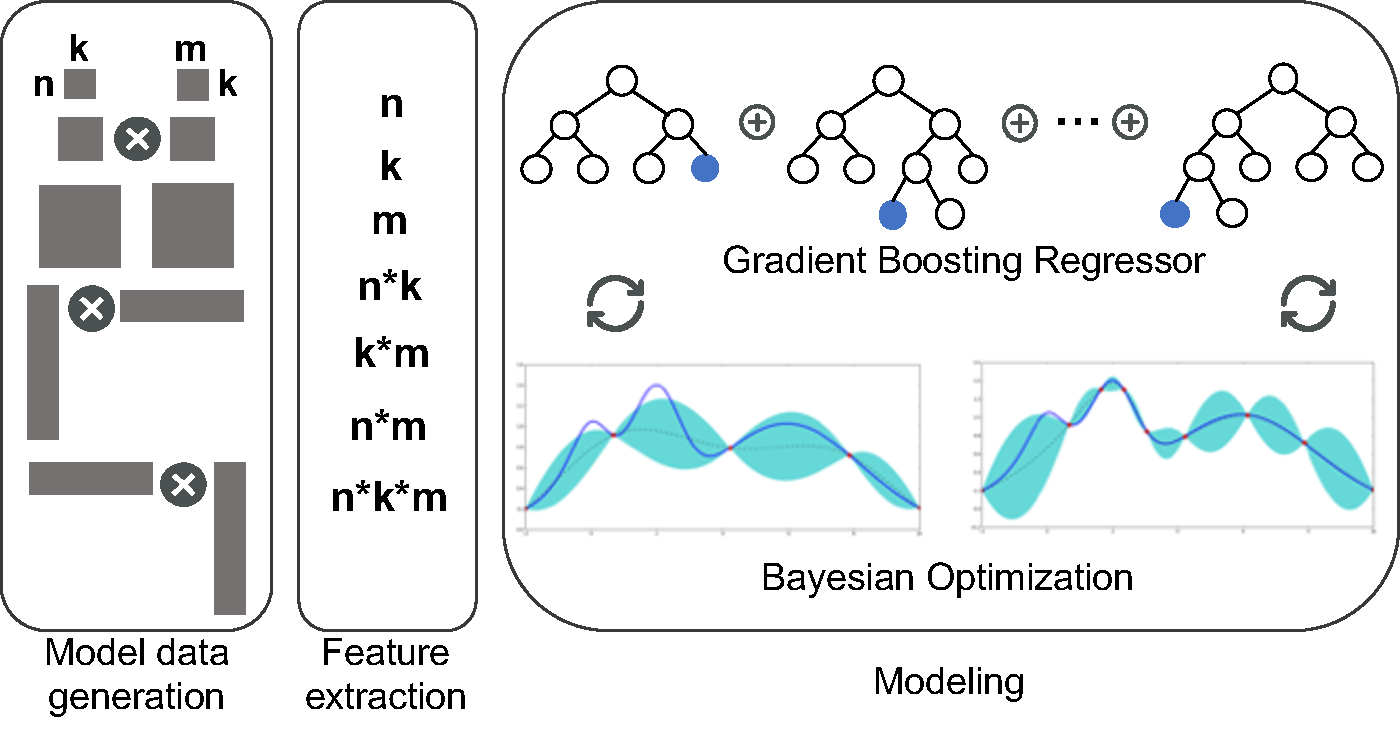
\includegraphics[width=0.5\textwidth]{figures/mpc-architecture.pdf}\caption{Architecture of MPC to predict various matrix multiplication performance}\label{fig:mpc-architecture}
\end{figure}

The opreation step of MPC is shown in Figure~\ref{fig:mpc-architecture} that is composed of train dataset generation, feature extraction, and modeling. In the modeling step, we iteratively apply bayesian optimization~\cite{bayesian-optimization} to find the optimally working hyper parameters of the chosen algorithm.

\subsection{Train Data Generation}
In the train data generation step, MPC performs offline profiling of various types and sizes of matrix multiplication to build a model to predict latency of arbitrary input dataset. A matrix multiplication task can be broadly grouped into square $\times$ square, long-thin $\times$ short-wide, and short-wide $\times$ long-thin matricies. To cover all the shapes and various sizes, MPC profiles the latency of synthetically generated left and right matricies. In the latency measurement, MPC utilizes Apach Spark WebUI REST API that provides various execution metricies in the JSON format.

To consider various cloud computing instances with distinct capacity, MPC adopts OpenBLAS to conduct computation on CPU and NVBLAS to conduct computation on instances that equip GPU devices. To allow Spark to interact with the hardware-optmized linear algebra libraries, we use netlib-java as proposed in~\cite{fatman-littleboy}.

\subsection{Feature Extraction}
As shown in Section~\ref{sec:overhead-modeling}, overheads of matrix multiplication in a distributed comptuing environments encompass various sources of resources. In order to account for such diverse overheads, MPC propose to utilize the dimension of input matrix blocks and the products, namely $n$, $m$, $k$, $n \times m$, $n \times k$, $k \times m$, and $n \times k \times m$, as features to model the performance. With $n \times m$ term, we can consider the size of output matrix, $n \times k$ and $k \times m$ terms represent the size of left and right matrix blocks size that impacts network and IO disk overhead. The $n \times k \times m$ term represents the total number of multiply operations.

Different from MPC, previous works that focus on predicting the performance of data mining tasks on cloud computing resources used a scale-based sampling mechanism as an input feature for prediction~\cite{ernest, cherrypick, paris}. They generally apply sampling at the input dataset by selecting very small portion and measure performance using the subset of dataset. Using the outcomes from the sample dataset, different algorithms apply distinct preditive algorithms, such as non negative linear equation (Ernest~\cite{ernest}), bayesian optimization (Cherrypick~\cite{cherrypick}), and random forest (PARIS~\cite{paris}), to make prediction. However, the scale-based sampling mechanism cannot capture the complex nature of distributed matrix muliplication, and it considers either $n$ or $m$ based on the sampling method. In the evaluation section, we demonstrate the superior performance of MPC due to the rich set of features.

\subsection{Modeling}
In the modeling step, MPC builds a model to represent the performance of multiplying various matricies. This step is composed of model build and hyper parameter search; MPC utilizes Gradient Boosting~\cite{gradient-boosting} regressor for model build step and Bayesian Optimization~\cite{bayesian-optimization} to find the optimal parameters to run GB method.


% Graidient boostring overview

Gradient Boosting is a flexible non-parametric statistical learning approach for classification and regression. The main idea of boosting is to add new models to the ensemble increasingly. A GB model is fitted in a forward stage-wise pattern; at each stage, a new weak, base-learner model is fit to the residual of the current model. In the case of least squares loss, The residual is proportional to the gradient of the loss function with regard to the ongoing model. It starts by fitting the first base model to the original target. the next base model is fitted on the residuals of the first stage. The final model is the sum of predictions of all individual base models. It is greatly customizable to the particular needs of the application with respect to different loss functions. It also automatically identifies non-linear feature interactions.
% Bayesian optimization overview

%The purpose of the modeling is estimating the execution latency when processing matrix multiplication application. To reduce the uncertainty of a non-linear interaction model and consider the noisy data in the cloud environment, we utilize~\textit{random forests} for modeling. 

%Random forests are a combination of tree predictors such that each tree depends on the values of a random vector sampled independently and with the same distribution for all trees in the forest.~\cite{random-forest}  Each tree is constructed with random subset of the training data. This lets each tree focus on a different chosen input variables which enhances the RF robustness to noisy data and screens the unimportant features. 

%To further improve the accuracy of prediction model, we leverage Bayesian Optimization, which is a framework to tune parameters of MI estimators. Bayesian optimization works by constructing a posterior distribution of functions that best illustrates the function you want to optimize. By using BO, the resulting relative error is below 7\text{\%} which is 2\text{\%} improvement regarding certainty of prediction model.

\section{Evaluation}{\label{sec:eval}}
In this section, we evaluate the performance of MPC thoroughly from the perspective of input matrix variability and cloud instance type diversity. Applying gradient boosting algorithm with the proposed features outperforms linear regressor by showing XY\% more prediction accuracy. Furthermore, by applying bayesian optimization to select optimal hyper-parameters of gradient boosting, we could improve the accuracy about XY\%. Evaluation of MPC with various cloud instance types demonstrates the effectiveness of MPC on a cloud computing environment. Finally, comparing MPC with Ernest~\cite{ernest}, the state-of-the-art machine learning performance predictor on cloud, shows that MPC has about XY\% more accuracy in predicting matrix multiplication latency.

\subsection{Setup}
To make diverse matrix multiplication scenarios for training and evaluation, we varied the number of rows and columns of left and right matricies from 128 to 800,000. Within the range, we generate XYZ(numnber of dataset) cases of square $\times$ square, long-thin $\times$ short-wide, and short-wide $\times$ long-thin matricies\footnote{test input cases - bit.ly/xyz}. The matrix multiplication is performed with Apach Spark and MLLib library with a version of 2.2.0. Multiplication of each matrix size is executed five times, and the average value is used to represent the latency of the size. A spark cluster is deployed to AWS EC2 by using \textit{spark-ec2} library\footnote{https://github.com/kmu-leeky/spark-ec2} with four \textit{R2.2xlarge} instances, unless otherwise stated. Each EC2 instance has hardware-optimized linear algebra library installed, namely NVBlas for a GPU instance (\textit{g2.2xlarge}) and OpenBlas for other instances. For matrix multiplication modeling and evaluation, we use \textit{scikit-learn} 0.18.1 with \textit{Python} 2.7.12.

\subsection{MPC Performance Evaluation}
\textbf{feature importance}: MPC proposes to use various combinations of left and right matrix block sizes as features to model complex mechanism of distributed matrix multiplication. To assess the impact of features in the model, we show the relative importance of features that are calculated by counting the number of times a feature is selected for splitting, and each split is weighted by the improved performance~\cite{gb-feature-importance} in Figure~\ref{fig:feature-importance}. \emph{GradientBoostingRegressor} method is performed 100 times, and the average importance value is shown with the minimum and maximum value in the error bar. The total number of multiply operation ($lr \times lc \times rc$) term is the dominant feature (0.41) as people generally expect. However, a feature that represents the shuffle overhead ($lr \times lc + rr \times rc$) is also a dominant factor (0.26) for the overall latency in the distributed matrix multiplication. The output size ($lr \times rc$) also imposes non-negligible impact (0.1), and this observation corresponds to Figure~\ref{fig:different-matrix-shapes} that shows the performance might differ for the same matrix size but different shape and output size, e.g., long-thin $\times$ short-wide versus short-wide $\times$ long-thin.

\begin{figure}
  \centering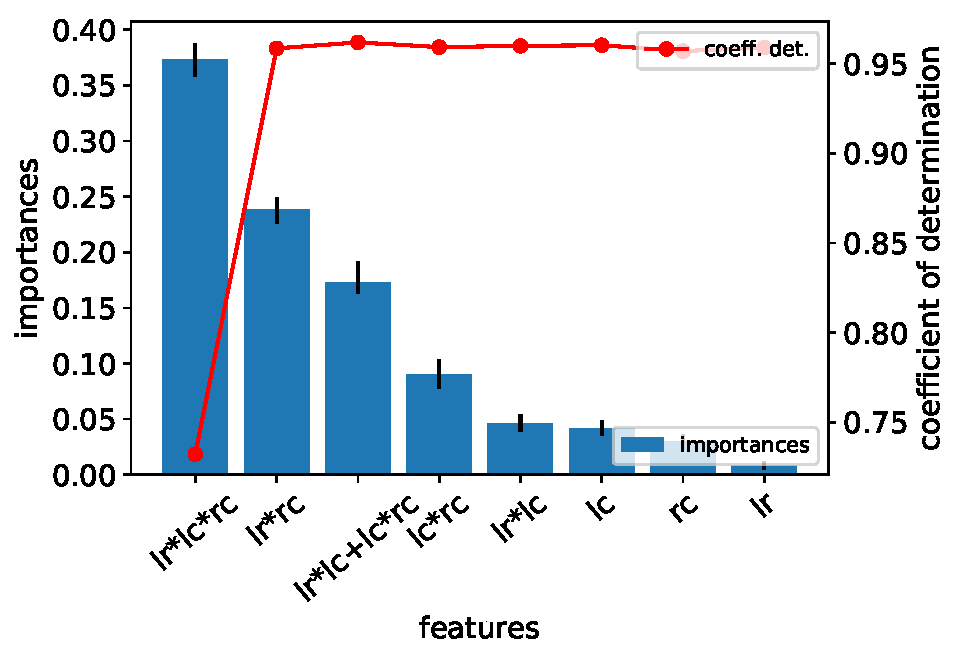
\includegraphics[width=0.45\textwidth]{figures/feature-importance.pdf}\caption{The relative importance of features for distributed matrix multiplication. The number of multiply operation, the shuffle overhead, and the output size are the three most important features.}\label{fig:feature-importance}
\end{figure}

% model comparison
% bayesian optimization
% prediction on cloud computing instances

\subsection{Comparison with Ernest}

\section{Related Work}\label{sec:relatedwork}
\textbf{Instance Recommendation:} Ernest~\cite{ernest} predicts performance for different VM and cluster sizes, targeting machine learning analytics applications. PARIS~\cite{Yadwadkar:2017:SBV:3127479.3131614} takes a hybrid online/offline approach, using a random forest model to predict application performance on various VM configurations based on features such as CPU utilization obtained from profiling. None of these systems consider the I/O overhead modeling in distributed cloud environments with arbitrary matrix shape which can affect matrix computation performance. 

%need taming
\textbf{Analyzing performance of data analytics frameworks:} While previous studies have analyzed how CPU, memory, network and storage resources affect Spark performance ~\cite{196352,li2014tachyon,ousterhout2015making} our work is the first to take consideration that I/O overhead can affect shape of the matrix. 

% need taming
% cloud computing performance prediction
% instance recommendation (Ernest, Paris, CCGrid 2017)
% Matrix multiplication performance and Spark + Matrix multiplication

\section{Conclusion and Future Work}
Conclusion~\cite{tr-spark}


\bibliographystyle{IEEEtranS}
\bibliography{abc2}
\end{document}
